\chapter{部分空間、射影演算子、そして測定としてのもつれ}

ベルの定理は二つの問いを残した。対の一方が擾乱され、吸収され、あるいは測定されたとき、もつれの何が残るのか。そして、正確には何が普通の相互作用を測定に変えるのか。その答えへの道は初等的な線形代数を通る。性質は部分空間であり、確率は射影演算子の期待値であり、測定装置は対象がもつれ合う相手となる別の量子系である。

\section{導入の動機：もつれ、局所性、測定}

一重項が二つの遠く離れた部分に分離され、一方の部分が測定されたとしよう。量子場の理論はそれらの間の仮想的な交換を記述しなければならないだろうか。遠方側では検出可能なことは何も起こらず、そこに使えるメッセージは届かない。磁場によって一方のスピンを局所的に回転させ、結合状態の詳細な形を変えることはできるが、もつれの量はその局所的操作の下で固定されたままである。もつれの定量的な尺度は後で扱う。当面の要点は、もはや相互作用しない二つの系は、一方の側に限定された操作によってのみでは、それらの共有するもつれを変えることができないということである。

\begin{classroomqa}
\lecturetimestamp{00:00:22}
\audiencequestion{空間的に離れた一重項の一方に対する測定は、他方との何らかの仮想的な交換を必要とするだろうか。}
\lecturerresponse{他方の側では検出可能な交換は起こらない。局所的操作は一方の因子を回転させ、結合状態が書かれる形を変えることはできるが、それ自体でメッセージを送ったり、隔たりを越えて共有されるもつれを変えたりすることはできない。}
\end{classroomqa}

そのことは、何が相手と見なされるかについて、より広い概念を強いる。もつれ合った対の一方がブラックホールに落ち込んでも、他方はもつれ合うのをやめない。それはブラックホールの自由度ともつれ合うようになり、蒸発の後には放出された輻射ともつれ合う。同じ考えにブラックホールは必要ない。もつれ合った対の一方を浴槽に落とし、水と激しく混ざり合わせてみよ。その個別の同一性は多体系状態の中で失われるかもしれないが、遠方の粒子は浴槽全体ともつれ合ったままであり、やがて逃げ出す蒸気ともつれ合う。

これは持続についての話だけではない。可逆性についての話でもある。相互作用がもつれを生成できるなら、相互作用は原理的にそれを元に戻すこともできる。もつれの解消は可能であるが、系が再び接触して相互作用するときに限られる。一方の向きに起こりうることは、他方の向きにも起こりうる。

\begin{classroomqa}
\lecturetimestamp{00:04:45}
\audiencequestion{もつれ合った対の両方のスピンが測定された場合、電子はもつれ合ったままであるか。一つの測定だけでもうそれらのもつれを解消できるか。}
\lecturerresponse{測定はそれらの相互のもつれを取り除くことができ、一つの測定で十分でありうる。その主張が単なる崩壊の断言ではなく何を意味するのかを見るには、観測を系と記録装置との間の相互作用として記述しなければならない。}
\end{classroomqa}

その問いが目標を定める。すなわち、観測、波束の崩壊、もつれを結びつけることである。しかしそれに近づく前に、議論が必要とする以上の重い道具立てを用いずに、部分空間と射影演算子についてより明快な説明が必要である。

\section{次元、線形従属、そして正規直交基底}

したがって当面は、ブラ、ケット、内積を備えた有限次元ベクトル空間にとどまる。サスキンドは可能な限り初等的に始める。彼は列ベクトルの成分を数えることによって次元を定義しない。彼はそれを抽象的 に定義する。ベクトル空間の次元とは、その中に見出しうる線形独立なベクトルの最大数である。

したがって、集合 \(\{|v_i\rangle\}\) は、関係
\begin{equation}
\sum_i c_i |v_i\rangle = 0
\end{equation}
がすべての係数 \(c_i\) をゼロにするとき、線形独立である。同値に、どのベクトルも他のベクトルの線形結合として書くことはできない。

ここで決定的なのは、直交性は独立性と同じものではないということである。三次元では、まったく直交していない三つのベクトルを持ちながら、それらが線形独立でありうる。重要なのは、それらの一つが他の二つから作れるかどうかである。一方、二次元平面では、その平面内の任意の第三のベクトルは最初の二つに線形従属でなければならない。

\begin{figure}[htbp]
\centering
\includegraphics[width=0.56\textwidth]{lecture_06_figure_02.png}
\caption{黒板に描かれた三つのベクトル。この講義はこの略図を用いて、直交性の考えと線形独立性の考えを区別し、次に平面では第三のベクトルが最初の二つに従属することを強調する。}
\lectureframe{00:09:35}
\end{figure}

\begin{figure}[htbp]
\centering
\begin{tikzpicture}[scale=1.2]
\draw[->] (0,0) -- (2.3,0);
\draw[->] (0,0) -- (2.0,2.0);
\draw[->] (0.35,0.95) -- (1.05,1.45);
\fill (0,0) circle (1.2pt);
\end{tikzpicture}
\caption{黒板のスケッチの最小限の再構成。厳密な係数の関係はこの枠組みだけでは定まらない。幾何学的な要点は、二次元平面では第三のベクトルは独立ではないということである。}
\end{figure}

これがこのスケッチの要点である。空間が二次元なら、線形独立なベクトルの最大数は二である。空間が三次元なら三である。より一般に、空間の次元が\(d\)なら、内積が与えられたとき、それを張る互いに直交する単位ベクトルを\(d\)個見つけることができる。これらが基底ベクトルである。Susskindはこの定理をここでは証明しないと明言している。彼が求めているのは結論だけである。すなわち、そのような基底が存在すれば、空間内のあらゆるベクトルをその基底で展開できるということである。

\begin{classroomqa}
\lecturetimestamp{00:10:58}
\audiencequestion{空間的自由度の数は状態空間の次元と同じなのか。}
\lecturerresponse{いいえ。部屋の中を運動する粒子は三つの空間座標をもつが、互いに直交する量子状態の数は膨大である。配位空間の次元とヒルベルト空間の次元は異なる概念であり、有限次元の例は論理を明快に示すために用いられているにすぎない。}
\end{classroomqa}

\section{基底展開、ダイアド、恒等作用素の分解}

ここで正規直交基底\(\{|n\rangle\}\)を選ぶ。ただし\(n=1,\dots,d\)とする。この時点の黒板はとりわけ明快で簡潔である。

\begin{figure}[htbp]
\centering
\includegraphics[width=0.62\textwidth]{lecture_06_figure_03.png}
\caption{正規直交基底と任意の状態の展開。}
\lectureframe{00:14:15}
\end{figure}

次のように書く。
\begin{align}
\langle m|n\rangle &= \delta_{mn}, \\
|\psi\rangle &= \sum_n a_n |n\rangle.
\end{align}
ここで\(\delta_{mn}\)はクロネッカーのデルタである。すなわち\(m=n\)のとき\(1\)であり、それ以外では\(0\)である。

\paragraph{導出の実演。}係数は基底への射影によって取り出される。左から\(\langle m|\)を掛けると、
\begin{align}
\langle m|\psi\rangle
  &= \sum_n a_n \langle m|n\rangle \\
  &= \sum_n a_n \delta_{mn} \\
  &= a_m.
\end{align}
したがって係数は単に
\begin{equation}
a_m = \langle m|\psi\rangle.
\end{equation}
である。係数は通常の複素数なので、ケットのどちら側に置いても何も変わらない。

係数を展開に代入し直すと、
\begin{equation}
|\psi\rangle = \sum_n |n\rangle \langle n|\psi\rangle.
\end{equation}
が得られる。これは、対象\(|n\rangle\langle n|\)、より一般には\(|a\rangle\langle b|\)を作用素として読むべきであることを示唆している。まさにこれが次の一手である。ダイアドは
\begin{equation}
\bigl(|a\rangle\langle b|\bigr)|\psi\rangle = \langle b|\psi\rangle\,|a\rangle.
\end{equation}
のように作用する。ブラは複素数を取り出し、ケットは結果として得られる方向を与える。これがSusskindのベクトルから作用素への低技術的な道筋である。

ここで先ほどの展開を作用素の観点から読む。
\begin{equation}
|\psi\rangle = \left(\sum_n |n\rangle\langle n|\right)|\psi\rangle
\end{equation}
がすべての\(|\psi\rangle\)について成り立つので、括弧内の作用素は恒等作用素でなければならない。
\begin{equation}
\sum_n |n\rangle\langle n| = I.
\end{equation}
これが恒等作用素の分解である。

\begin{figure}[htbp]
\centering
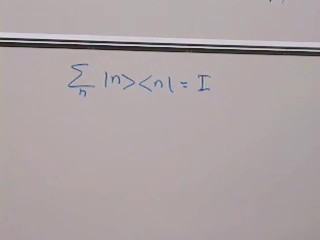
\includegraphics[width=0.60\textwidth]{lecture_06_figure_07.png}
\caption{完成した黒板の恒等作用素の分解。}
\lectureframe{00:18:30}
\end{figure}

\begin{classroomqa}
\lecturetimestamp{00:18:39}
\audiencequestion{恒等作用素の分解に現れるベクトルは基底でなければならないのか。}
\lecturerresponse{はい。この導出では規格化と相互直交性の両方を用いており、和は完全な基底にわたって取らなければならない。任意のベクトルの集まりでは恒等作用素を分解できない。}
\end{classroomqa}

恒等作用素それ自体は空間全体への射影作用素である。あらゆるベクトルは\(I\)の固有ベクトルであり、すべての固有値は\(+1\)である。

\begin{classroomqa}
\lecturetimestamp{00:19:14}
\audiencequestion{恒等作用素の分解は、あらゆるベクトルが固有値一をもつと言っているのか。}
\lecturerresponse{はい、恒等作用素についてはそうである。恒等作用素は、あらゆるベクトルがその固有ベクトルであり、すべての状態について\(I|\psi\rangle=|\psi\rangle\)であるという点で例外的である。}
\end{classroomqa}

\section{性質としての部分空間と射影作用素}

その道具立てを手にすると、講義は中心となる概念的な修正を行う。\(k=\lambda\)のような性質は、一般には一つのベクトルではない。それは部分空間全体である。

\(k\)をエルミートな観測量とし、
\begin{equation}
k|A\rangle = \lambda |A\rangle, \qquad
k|B\rangle = \lambda |B\rangle,
\end{equation}
が成り立つとする。ただし\(|A\rangle\)と\(|B\rangle\)は線形独立である。このとき任意の線形結合は同じ固有値をもつ。
\begin{align}
k\bigl(\alpha|A\rangle+\beta|B\rangle\bigr)
  &= \alpha k|A\rangle + \beta k|B\rangle \\
  &= \alpha \lambda |A\rangle + \beta \lambda |B\rangle \\
  &= \lambda\bigl(\alpha|A\rangle+\beta|B\rangle\bigr).
\end{align}
したがって\(\lambda\)に対する固有空間は加法とスカラー倍について閉じている。それはベクトル部分空間である。

講義の最初の具体的な例は二スピン系である。状態
\begin{equation}
|ud\rangle,\qquad |uu\rangle
\end{equation}
は第二スピンの値が異なるが、第一スピンの値は同じである。どちらの場合も第一スピンは上である。したがってこれらは、第一スピンについて\(\sigma_3=+1\)となる部分空間を張る。

\begin{figure}[htbp]
\centering
\includegraphics[width=0.46\textwidth]{lecture_06_figure_04.png}
\caption{第一スピンが上である二つの二スピン状態。}
\lectureframe{00:23:27}
\end{figure}

これが保持すべき要点である。性質は必ずしも一つの状態ではない。それは同じ固有値をもつ状態の集まり全体である。

黒板に一瞬現れる記法の混乱を避けるため、特定の固有ベクトルには大文字 \(A,B,\dots\) を用い、小文字 \(a,b,\dots\) は固有部分空間の正規直交基底にわたる和の添字として用いることにする。\(\{|a\rangle\}\) が部分空間 \(k=\lambda\) のそのような基底であれば、その部分空間への射影演算子は
\begin{equation}
\Pi_{k=\lambda}=\sum_a |a\rangle\langle a|.
\end{equation}
である。これはその部分空間に制限された恒等演算子にほかならない。\(|\psi\rangle\) がすでにその部分空間内にあれば、射影演算子はそれを変えずに返す。\(|\psi\rangle\) が部分的に外側にあれば、射影演算子は直交する残りの部分を捨て、内側の成分のみを保つ。

\section{確率の公準、両立する性質、およびベルの復習}

性質が部分空間として再解釈されると、確率の公準は最も明快な形をとる。\(|\psi\rangle\) が規格化されているとき、それが性質 \(k=\lambda\) をもつ確率は
\begin{equation}
P(k=\lambda)=\langle\psi|\Pi_{k=\lambda}|\psi\rangle.
\end{equation}

\begin{figure}[htbp]
\centering
\includegraphics[width=0.58\textwidth]{lecture_06_figure_05.png}
\caption{\(k=\lambda\) 固有部分空間への射影演算子。黒板上の配置はすでに次の手順を準備している。すなわち、射影演算子を \(\langle\psi|\) と \(|\psi\rangle\) で挟むのである。}
\lectureframe{00:31:09}
\end{figure}

射影演算子のダイアド形を代入すると、
\begin{align}
P(k=\lambda)
  &= \left\langle \psi \left| \sum_a |a\rangle\langle a| \right| \psi \right\rangle \\
  &= \sum_a \langle\psi|a\rangle\langle a|\psi\rangle \\
  &= \sum_a |\langle a|\psi\rangle|^2.
\end{align}
これはまさに講義の解釈である。すなわち、その性質に対する全確率は、その性質が生じうるすべての直交する仕方の確率の和である。

二スピン系において第一のスピンが上向きである場合、関連する部分空間は\(|uu\rangle\)と\(|ud\rangle\)によって張られるので、
\begin{equation}
\Pi_{\sigma_3=+1}=|uu\rangle\langle uu|+|ud\rangle\langle ud|.
\end{equation}
となる。講義の略記法では、これは
\begin{equation}
\Pi_{\sigma_3=+1}=\frac{1+\sigma_3}{2},
\end{equation}
とも書かれ、第二のスピン上の恒等演算子は省略されている。

\begin{classroomqa}
\lecturetimestamp{00:33:04}
\audiencequestion{可観測量、性質、射影演算子の違いは何か。}
\lecturerresponse{可観測量はエルミート演算子 \(k\) である。性質 \(k=\lambda\) はその固有部分空間によって表され、\(k\) を測定すれば必ず \(\lambda\) が得られることを意味する。射影演算子 \(\Pi_{k=\lambda}\) はその部分空間を分離し、その期待値がその性質が存在する確率を与える。}
\end{classroomqa}

\begin{classroomqa}
\lecturetimestamp{00:34:07}
\audiencequestion{縮退した固有ベクトル \(A\) と \(B\) はすでに直交していなければならないのか、またそれらは空間全体の基底なのか。}
\lecturerresponse{元の固有ベクトルは直交している必要はないが、それらの固有部分空間内で常に正規直交基底を選ぶことができる。それはその部分空間の基底にすぎず、空間全体を張るには追加の直交方向が必要である。各部分空間の基底ベクトルへの射影を足し合わせると、その部分空間への射影が得られる。}
\end{classroomqa}

\begin{classroomqa}
\lecturetimestamp{00:35:33}
\audiencequestion{\(k|A\rangle=\lambda|A\rangle\) における記号 \(a\) は、射影演算子で和をとる \(a\) と同じものを意味するのか。}
\lecturerresponse{いいえ。前者は特定の固有ベクトルを表すのに対し、和の下の添字は固有部分空間の正規直交基底のすべてのベクトルにわたって動く。異なる記法によって、固定されたラベルがダミーの和の添字と取り違えられるのを防ぐ。}
\end{classroomqa}

\begin{classroomqa}
\lecturetimestamp{00:37:15}
\audiencequestion{射影演算子の公式における内積は確率か、それとも確率振幅か。}
\lecturerresponse{各 \(\langle a|\psi\rangle\) は振幅である。その複素共役を掛けると確率が得られ、\(k=\lambda\) を実現する直交する仕方にわたってそれらの確率を足し合わせると、その性質に対する全確率が得られる。}
\end{classroomqa}

次に講義は、性質をどのように組み合わせるかを問う。可換な射影演算子 \(P_k\) と \(P_\ell\) で表される2つの両立する性質があるとする。講義の言葉では、AND の命題は積で表される。
\begin{equation}
\Pi_{k=\lambda\,\wedge\,\ell=\mu}=P_kP_\ell=P_\ell P_k.
\end{equation}
論理は単純である。\(P_k|\psi\rangle\) は \(k=\lambda\) 部分空間にある。演算子が可換なので \(P_\ell P_k|\psi\rangle=P_kP_\ell|\psi\rangle\) であり、したがって同じベクトルは \(\ell=\mu\) 部分空間にもある。よって積は同時的な性質への射影となる。対応する確率は
\begin{equation}
P(k=\lambda,\ell=\mu)=\langle\psi|P_kP_\ell|\psi\rangle.
\end{equation}

その議論の最初の段階は、それ自体で示す価値がある。任意の状態に対して
\begin{equation}
k\bigl(P_k|\psi\rangle\bigr)=\lambda P_k|\psi\rangle,
\end{equation}
であるから、\(P_k|\psi\rangle\) は \(k=\lambda\) 固有部分空間にある。\(P_k\) と \(P_\ell\) が可換なら、積はどちらの射影演算子を左に置いても書けるので、両方の部分空間に属する。

\begin{figure}[htbp]
\centering
\includegraphics[width=0.44\textwidth]{lecture_06_figure_06.png}
\caption{固有部分空間内のベクトルとしての射影された状態。}
\lectureframe{00:41:57}
\end{figure}

\begin{figure}[htbp]
\centering
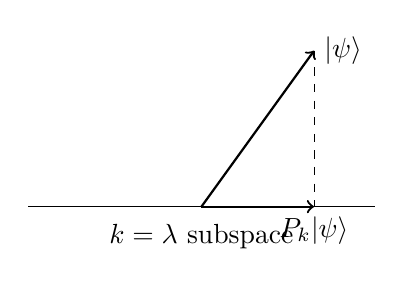
\begin{tikzpicture}[scale=1.1]
\draw (-2,0) -- (2,0);
\draw[->,thick] (0,0) -- (1.3,1.8) node[right] {$|\psi\rangle$};
\draw[dashed] (1.3,1.8) -- (1.3,0);
\draw[->,thick] (0,0) -- (1.3,0) node[below] {$P_k|\psi\rangle$};
\node at (0,-0.35) {$k=\lambda$ subspace};
\end{tikzpicture}
\caption{任意のベクトルを \(k=\lambda\) 固有部分空間へ射影すること。}
\end{figure}

\begin{figure}[htbp]
\centering
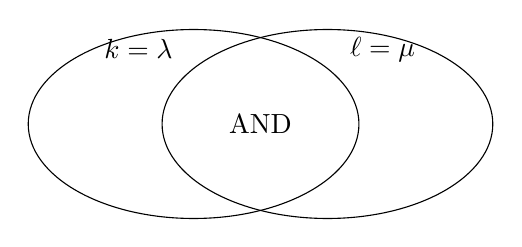
\begin{tikzpicture}[scale=1.0]
\draw (0,0) ellipse (2.1 and 1.2);
\draw (1.7,0) ellipse (2.1 and 1.2);
\node at (-0.7,0.95) {$k=\lambda$};
\node at (2.4,0.95) {$\ell=\mu$};
\node at (0.85,0) {AND};
\end{tikzpicture}
\caption{可換な射影演算子に対する AND 命題の背後にある交差部分空間の描像の再構成。}
\end{figure}

\begin{figure}[htbp]
\centering
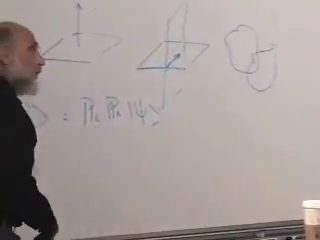
\includegraphics[width=0.66\textwidth]{lecture_06_figure_08.png}
\caption{可換な射影演算子が同時固有部分空間を選び出すという黒板での議論。}
\lectureframe{00:45:20}
\end{figure}

\begin{classroomqa}
\lecturetimestamp{00:44:42}
\audiencequestion{同時に成り立つ性質は、古典論理における共通部分と同じものか。}
\lecturerresponse{はい。可換な射影演算子に対して、\(P_kP_\ell\) は二つの固有部分空間の共通部分への射影である。共通部分が零ベクトルのみを含むなら、両方の性質をもつ非零状態は存在しない。}
\end{classroomqa}

念のため述べると、両立するOR部分空間への射影演算子は
\begin{equation}
P_{k\lor\ell}=P_k+P_\ell-P_kP_\ell .
\end{equation}
である。選択肢が互いに排他的であるとき、\(P_kP_\ell=0\) であり、これは和 \(P_k+P_\ell\) に帰着する。この減算は、二つの部分空間が重なるときには常に不可欠である。なぜなら、それらの共通部分を二重に数えてはならないからである。

次に、両立性そのものが物理的な例に結び付けられる。二スピン系では、第一のスピンの任意の成分 \(\sigma_i\) は第二のスピンの任意の成分 \(\tau_j\) と可換である：
\begin{equation}
[\sigma_i,\tau_j]=0.
\end{equation}
対照的に、同じスピンの異なる成分は可換でない：
\begin{equation}
[\sigma_1,\sigma_3]\neq 0.
\end{equation}
だからこそ、二つの離れたスピンのそれぞれについて一つの成分を測定することはできるが、同じスピンの二つの異なる成分を同時に測定することはできない。

\begin{classroomqa}
\lecturetimestamp{00:46:12}
\audiencequestion{両立する観測量の具体的な例は何か。}
\lecturerresponse{第一のスピンに作用する任意の演算子は、第二のスピンに作用するすべての演算子と可換である。なぜなら、それらは異なるテンソル因子に作用するからである。位置の成分 \(x,y,z\) も別の両立する族である。対照的に、同じスピンの二つの異なる成分、あるいは位置とその共役運動量は可換でない。}
\end{classroomqa}

\begin{classroomqa}
\lecturetimestamp{00:47:26}
\audiencequestion{部分系とは異なる粒子を意味しなければならないのか。}
\lecturerresponse{いいえ。それは独立に指定された自由度の集合を意味する。異なる粒子は最も単純なテンソル因子を与えるが、一つの粒子の異なる自由度も、その演算子構造が許すときには別々に扱うことができる。}
\end{classroomqa}

\begin{classroomqa}
\lecturetimestamp{00:48:37}
\audiencequestion{異なる部分系上のこれほど多くの演算子が可換なら、単純な非両立対は何か。}
\lecturerresponse{同じスピンの二つの成分が標準的な例を与える：\(\sigma_1\) と \(\sigma_3\) は可換でないので、いかなる装置も両方に同時に確定した値を割り当てることはできない。非零の行列交換子がその代数的な判定基準である。}
\end{classroomqa}

ここでSusskindはベルの定理を再訪する。彼は前回の講義の計算をやり直すのではない。新しい言語でその論理を組み直すのである。確率の形で表した古典的不等式は
\begin{equation}
P(A\wedge \neg B)+P(B\wedge \neg C)\ge P(A\wedge \neg C).
\end{equation}
である。これは古典的集合論の定理であり、量子力学の定理ではない。一重項状態では、スピンは任意の共通軸に沿って反平行であるため、第一のスピンについてのNOT文は、第二のスピンについての対応する肯定的文に置き換えることができる。それにより、この不等式を二スピン系の結合的性質についての文として書き換えることができる。

触れられていない因子上の恒等演算子を省略すると、講義に現れる単一性質の射影演算子は
\begin{equation}
\frac{1+\sigma_3}{2},\qquad
\frac{1+\frac{\tau_1+\tau_3}{\sqrt2}}{2},\qquad
\frac{1+\frac{\sigma_1+\sigma_3}{\sqrt2}}{2},\qquad
\frac{1+\tau_1}{2}.
\end{equation}
である。したがって、関連する三つの結合射影演算子は
\begin{align}
\Pi_1 &= \frac{1+\sigma_3}{2}\,\frac{1+\frac{\tau_1+\tau_3}{\sqrt2}}{2}, \\
\Pi_2 &= \frac{1+\frac{\sigma_1+\sigma_3}{\sqrt2}}{2}\,\frac{1+\tau_1}{2}, \\
\Pi_3 &= \frac{1+\sigma_3}{2}\,\frac{1+\tau_1}{2}.
\end{align}
となる。

\begin{figure}[htbp]
\centering
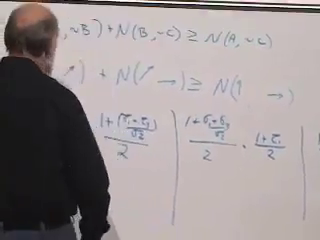
\includegraphics[width=0.68\textwidth]{lecture_06_figure_09.png}
\caption{三つの分析器の選択を、一スピンの射影演算子の積として書いたもの。}
\lectureframe{01:01:45}
\end{figure}

講義では、一重項をよく知られた規格化されていない黒板の形で述べる：
\begin{equation}
|\Psi_{\mathrm{singlet}}\rangle \propto |ud\rangle-|du\rangle.
\end{equation}
ここでは比例記号で十分である。論理にとって重要なのは状態そのもの、特に相対符号であり、全体の規格化ではない。一重項状態で \(\langle \Pi_1\rangle+\langle \Pi_2\rangle\) を \(\langle \Pi_3\rangle\) に対して評価すると、前回の講義で得られた破れが得られる。重要な結論は、Susskindが口頭で強調するものである：量子力学は変装した古典的集合論ではない。

\begin{classroomqa}
\lecturetimestamp{00:52:31}
\audiencequestion{スピンアップとスピンダウンが直交するなら、マイナス符号は一方のケットが他方の負であることを意味するのか。}
\lecturerresponse{いいえ。\(|u\rangle\) と \(|d\rangle\) は異なる直交ベクトルである。相対符号は \(|ud\rangle-|du\rangle\) のような重ね合わせに属し、その物理的性質を変えうる。状態全体に掛かる全体符号のみが無意味である。}
\end{classroomqa}

\begin{classroomqa}
\lecturetimestamp{00:53:06}
\audiencequestion{ベルの不等式は、すべての量子状態とすべての性質の選択に対して破れるのか。}
\lecturerresponse{いいえ。多くの状態と多くの軸の選択が、特定のベルの不等式を満たす。破れは状態と選ばれた観測量の両方に依存する。中間角と最終角を変えると、このテストが非古典的相関を露わにするかどうかが変わる。}
\end{classroomqa}

\begin{classroomqa}
\lecturetimestamp{01:02:47}
\audiencequestion{特定の状態がこのベル不等式を破る場合、あるいはたまたま満たす場合、何が結論できるか。}
\lecturerresponse{破れは、観測された統計が導出で用いた古典的集合論理から生じ得ないことを証明する。選んだ一つの不等式を満たすことは、それ自体ではその状態を古典的にしない。なぜなら、別の性質の選択が破れを明らかにするかもしれないからである。}
\end{classroomqa}

\section{ベル以降の局所性}

射影演算子の計算は単なる記号遊びではない。一重項基底状態にある相関した対を繰り返し準備し、二つの構成要素を分離し、同一に準備された集団を三つの大きな群に分ける状況を想像せよ。第一の群は\(0^\circ\)と\(45^\circ\)の設定を測定し、第二の群は\(45^\circ\)と\(90^\circ\)の設定を、第三の群は\(0^\circ\)と\(90^\circ\)の設定を測定する。三つの群における頻度が、不等式に現れる三つの確率を推定する。

\begin{classroomqa}
\lecturetimestamp{01:04:30}
\audiencequestion{三つのベル確率は実際にはどのような実験配置を記述しているのか。}
\lecturerresponse{線源が同一に準備された多数のもつれ対を生成し、その二つの構成要素を離れた解析器へ送る。対を三つの集団に分け、各集団に解析器の方向の対応する対を用いる。同時結果を数えることで各確率を推定する。荷電粒子と反粒子は場によって分離できるが、実際のベルテストではしばしば代わりに光子が用いられる。}
\end{classroomqa}

\begin{classroomqa}
\lecturetimestamp{01:08:00}
\audiencequestion{古典的集合の証明は一つの母集団を用いた。三つの別々に測定された集団がそれをどのように検証できるのか。}
\lecturerresponse{この不等式は計数だけでなく確率についての主張でもある。三つの標本がすべて同じ準備手続きから引き出されているなら、それらの相対頻度は一つの共通の集団の三つの確率分布を推定する。同一の準備が不可欠な仮定である。}
\end{classroomqa}

そのベルの復習は、部屋にまだ漂っている物理的な不安へと直接つながる。相関が実在するなら、なぜそれを信号の送信に使えないのか。

\begin{classroomqa}
\lecturetimestamp{01:09:41}
\audiencequestion{なぜもつれた相関を超光速メッセージの送信に使えないのか。}
\lecturerresponse{各翼はそれぞれ、依然として制御不能なランダム系列を見る。相関は、二つの記録が通常の古典的チャネルを通じて比較されたときに初めて可視になる。それにもかかわらず、決定的なベルテストは選択と検出を、光信号が翼間を時間内に通過できないように配置し、それによって同時統計を生み出す局所的な通信機構を排除する。}
\end{classroomqa}

光信号が装置間を移動するのに十分な時間が経過するなら、相関それ自体は相対性理論と矛盾しない。単に気づかれていない通常の影響を発見しただけかもしれない。鋭い実験はその逃げ道を閉ざす。ベルの言葉では、相関を再現する隠れた変数の説明は非局所的でなければならないが、非局所的な依存は制御可能な超光速メッセージと同じものではない。

\begin{classroomqa}
\lecturetimestamp{01:12:18}
\audiencequestion{角運動量の保存はこの議論に本質的か。}
\lecturerresponse{いいえ。スピンは便利な二状態模型であり、神聖な要素ではない。必要なもつれた状態と代替の測定基底を持つ任意の二準位系の対が、同じ論理構造を示すことができる。}
\end{classroomqa}

この議論は講義を締めくくるものではない。次の転換のための地ならしをするものである。ベルは、量子力学が古典論理ではないことを我々に教えたが、次の問いは異なる。測定とは、操作的かつ数学的に何であり、干渉の物語にどのように入ってくるのか。

\section{有限状態の二重スリット、干渉、そしてもつれとしての測定}

講義はここで模型を変える。サスキンドは二重スリット実験へ向かうが、連続波動力学の完全な道具立てを持ち込むことなく同じベクトル空間の技術を使えるように、直ちにそれを有限状態の問題へ単純化する。彼は事実上、これが依然として二重スリット実験であり、ただ少数の基底状態に削ぎ落とされただけだと言う。

線源状態\(|0\rangle\)、二つのスリット状態\(|1\rangle\)と\(|-1\rangle\)、そしてスクリーン状態の集合\(|n\rangle\)がある。これらの\(|n\rangle\)は、異なるスクリーン位置が異なる配置であるため、正規直交である。講義はここで正規化を注意深く追跡しないことを明示的に選ぶ。ユニタリ性は後回しにされる。この段階で重要なのは線形性である。

\begin{figure}[htbp]
\centering
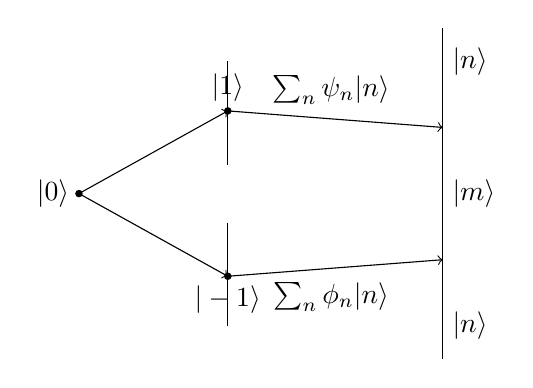
\begin{tikzpicture}[scale=1.05]
\fill (0,0) circle (1.3pt);
\node[left] at (0,0) {$|0\rangle$};

\draw (1.8,1.6) -- (1.8,0.35);
\draw (1.8,-0.35) -- (1.8,-1.6);
\fill (1.8,1) circle (1.3pt);
\fill (1.8,-1) circle (1.3pt);
\node[above] at (1.8,1) {$|1\rangle$};
\node[below] at (1.8,-1) {$|-1\rangle$};

\draw (4.4,2.0) -- (4.4,-2.0);
\node[right] at (4.4,1.6) {$|n\rangle$};
\node[right] at (4.4,0.0) {$|m\rangle$};
\node[right] at (4.4,-1.6) {$|n\rangle$};

\draw[->] (0,0) -- (1.8,1);
\draw[->] (0,0) -- (1.8,-1);
\draw[->] (1.8,1) -- (4.4,0.8);
\draw[->] (1.8,-1) -- (4.4,-0.8);

\node at (3.05,1.25) {$\sum_n \psi_n |n\rangle$};
\node at (3.05,-1.25) {$\sum_n \phi_n |n\rangle$};
\end{tikzpicture}
\caption{二重スリット実験の有限状態版：線源状態\(|0\rangle\)、二つのスリット状態\(|1\rangle\)と\(|-1\rangle\)、そしてスクリーン基底\(|n\rangle\)。}
\end{figure}

\begin{figure}[htbp]
\centering
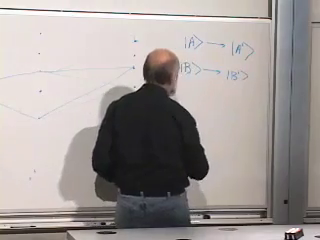
\includegraphics[width=0.68\textwidth]{lecture_06_figure_10.png}
\caption{線形な発展則\(A\to A'\)、\(B\to B'\)の隣にある有限の位置格子。}
\lectureframe{01:18:00}
\end{figure}

対称性により、源は2つのスリット状態の等振幅の重ね合わせへと発展する：
\begin{equation}
|0\rangle \longrightarrow |1\rangle+|-1\rangle.
\end{equation}
ここで、上側のスリット状態が
\begin{equation}
|1\rangle \longrightarrow \sum_n \psi_n |n\rangle,
\end{equation}
へと発展し、下側のスリット状態が
\begin{equation}
|-1\rangle \longrightarrow \sum_n \phi_n |n\rangle.
\end{equation}
へと発展するとしよう。ここでの矢印は時間発展を意味し、同一時刻における状態の等号ではない。線形性により、
\begin{equation}
|1\rangle+|-1\rangle \longrightarrow \sum_n (\psi_n+\phi_n)|n\rangle.
\end{equation}
これが鍵となる規則である。振幅は確率が作られる前に加算される。

\begin{classroomqa}
\lecturetimestamp{01:21:59}
\audiencequestion{スリット状態\(|1\rangle\)が、同じく整数\(n\)でラベル付けされた状態に変わりうるのはなぜか。これらのケットは同じ場所と同じ時刻にあるのか。}
\lecturerresponse{ラベルは異なる時間スライスを指している。\(|1\rangle\)は上側のスリットにある電子を表すのに対し、右辺の\(|n\rangle\)はスクリーン上の可能な後の位置を表す。矢印は時間発展であり、同時刻の配置の間の等号ではない。}
\end{classroomqa}

\begin{classroomqa}
\lecturetimestamp{01:25:30}
\audiencequestion{振幅は規格化されるべきか、また物理的な単位を持つのか。}
\lecturerresponse{完全な発展は全確率を保存しなければならない。それがユニタリ性である。ここでは経路振幅の加算と相殺だけが重要なので、共通の規格化因子は省略されている。状態を規格化する際に、任意のスケール因子を復元できる。}
\end{classroomqa}

したがって、スクリーン上の位置\(m\)に到達する確率は
\begin{align}
P_m &= |\psi_m+\phi_m|^2 \\
    &= |\psi_m|^2 + |\phi_m|^2 + \psi_m^*\phi_m + \phi_m^*\psi_m.
\end{align}
最初の2つの項は、古典的な推論が生み出したであろうものである。最後の2つの項が干渉項である。

\begin{figure}[htbp]
\centering
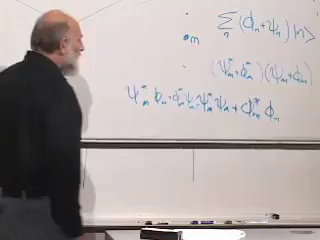
\includegraphics[width=0.68\textwidth]{lecture_06_figure_11.png}
\caption{スクリーン上の振幅と、黒板上でのその4項からなる確率展開。}
\lectureframe{01:29:20}
\end{figure}

スクリーン上の対称な点を\(m=0\)と呼ぶと、対称性から\(\psi_0=\phi_0\)が示唆される。すると
\begin{equation}
P_0 = |\psi_0+\phi_0|^2 = |2\psi_0|^2 = 4|\psi_0|^2.
\end{equation}
両方のスリットを開けると、その点での1スリット確率の4倍が生じ、2倍ではない。これが建設的干渉である。

次に位相シフトを挿入し、\(\phi_0=-\psi_0\)とする。すると
\begin{equation}
P_0 = |\psi_0-\psi_0|^2 = 0.
\end{equation}
各スリットは単独ではその点への到達を許すが、両方を一緒に開けるとそこへの到達を不可能にすることがある。これが破壊的干渉である。Susskindはこれがいかに奇妙であるかを明示的に強調している。彼にとっては、これはBellと同じくらい奇妙である。

\begin{classroomqa}
\lecturetimestamp{01:33:14}
\audiencequestion{位相シフターやスリットの選択が、電子がすでに飛行している後にのみ変更されたらどうなるか。もう一方のスリットはそれについて知るための時間を必要とするのか。}
\lecturerresponse{答えは、正確な時空配置と、電子が装置の変更された部分に出会うかどうかに依存する。量子力学は実際の設定を通じて状態を発展させる。確率は依然として、適用可能な振幅を加算することから得られる。遅延選択の提案は、局所性の主張を評価できるようになる前に、厳密に指定されなければならない。}
\end{classroomqa}

ここで装置を導入する。追加の2状態系が1つあり、スピンは初期に状態\(|d\rangle\)にある。電子が上側のスリットを通ると、そのスピンは\(|u\rangle\)へと反転する。下側のスリットを通る場合、スピンは変わらないままである。初期の合成状態は\(|0,d\rangle\)であり、最初の更新規則は
\begin{equation}
|0,d\rangle \longrightarrow |1,u\rangle + |-1,d\rangle.
\end{equation}
となる。この1行が、講義における測定の意味のすべてである。電子の位置は、装置に蓄えられた記録とエンタングルしてしまったのである。

\begin{figure}[htbp]
\centering
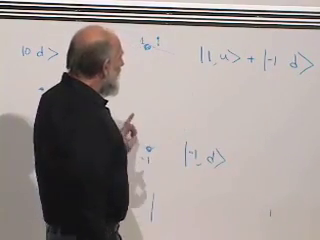
\includegraphics[width=0.66\textwidth]{lecture_06_figure_12.png}
\caption{検出器スピンは、その上向きと下向きの記録を2つのスリットの選択肢と相関させる。}
\lectureframe{01:44:10}
\end{figure}

\begin{classroomqa}
\lecturetimestamp{01:40:20}
\audiencequestion{両方のスリットに検出器が必要なのだろうか？}
\lecturerresponse{信頼できる検出器は1台で十分である。上側のスリットを通ったことをそれが記録すれば、記録が変化していないことから下側の選択肢が特定される。ただし、透過したすべての電子が2つの開口のいずれかを通らなければならない場合に限る。2台目の検出器を置くことも可能だが、原理を変えることなく別のサブシステムを追加するだけである。}
\end{classroomqa}

\begin{classroomqa}
\lecturetimestamp{01:40:51}
\audiencequestion{電子は両方のスリットを通ると言ってはいけないのか。}
\lecturerresponse{経路の記録がなければ、状態はコヒーレントな重ね合わせであり、遡及的な経路の事実は得られない。完全なwhich-path測定があれば、装置は各回の実行で一方の選択肢または他方を記録する。両方の選択肢を通じて持続するのは状態振幅であり、別々に観測された2つの電子の軌道ではない。}
\end{classroomqa}

\begin{figure}[htbp]
\centering
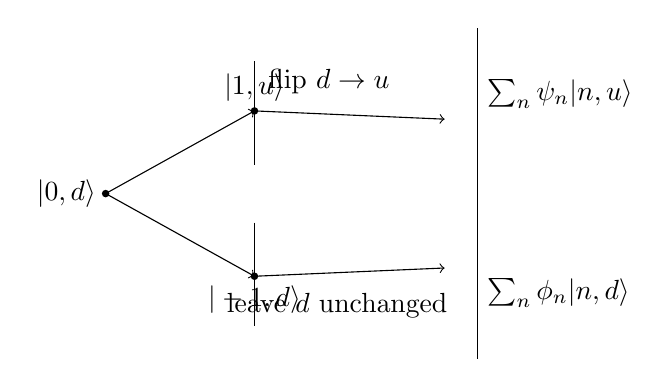
\begin{tikzpicture}[scale=1.05]
\fill (0,0) circle (1.3pt);
\node[left] at (0,0) {$|0,d\rangle$};

\draw (1.8,1.6) -- (1.8,0.35);
\draw (1.8,-0.35) -- (1.8,-1.6);
\fill (1.8,1) circle (1.3pt);
\fill (1.8,-1) circle (1.3pt);
\node[above] at (1.8,1) {$|1,u\rangle$};
\node[below] at (1.8,-1) {$|-1,d\rangle$};

\draw (4.5,2.0) -- (4.5,-2.0);
\node[right] at (4.5,1.2) {$\sum_n \psi_n |n,u\rangle$};
\node[right] at (4.5,-1.2) {$\sum_n \phi_n |n,d\rangle$};

\draw[->] (0,0) -- (1.8,1);
\draw[->] (0,0) -- (1.8,-1);
\draw[->] (1.8,1) -- (4.1,0.9);
\draw[->] (1.8,-1) -- (4.1,-0.9);

\node at (2.7,1.35) {flip \(d\to u\)};
\node at (2.8,-1.35) {leave \(d\) unchanged};
\end{tikzpicture}
\caption{検出器スピンとのエンタングルメントとしての測定。上側の経路は装置のスピンを反転させ、下側の経路はそれを変えないままにする。}
\end{figure}

講義と同様に、スクリーンに至るまでの間、スピンにはそれ以上何も起こらないと仮定する。すると
\begin{align}
|1,u\rangle &\longrightarrow \sum_n \psi_n |n,u\rangle, \\
|-1,d\rangle &\longrightarrow \sum_n \phi_n |n,d\rangle.
\end{align}
したがって、両方のスリットを開いたときの最終状態は
\begin{equation}
|\Psi_{\mathrm{final}}\rangle
  = \sum_n \psi_n |n,u\rangle + \sum_n \phi_n |n,d\rangle.
\end{equation}
これは1個の電子だけの状態の重ね合わせではない。電子と装置のエンタングル状態である。

\begin{figure}[htbp]
\centering
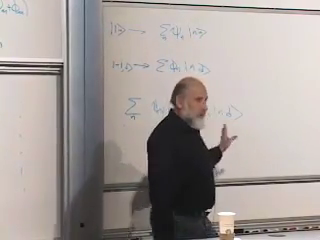
\includegraphics[width=0.68\textwidth]{lecture_06_figure_13.png}
\caption{2つの経路の振幅は、直交する装置の記録を伴ってスクリーンに到達する。}
\lectureframe{01:47:35}
\end{figure}

位置\(m\)への到達確率を計算する最も明快な方法は、電子の部分系に対するその位置への射影演算子を用いることである：
\begin{equation}
\Pi_m = |m\rangle\langle m|\otimes I_{\mathrm{spin}}.
\end{equation}
\(\Pi_m\)を最終状態に作用させると
\begin{equation}
\Pi_m |\Psi_{\mathrm{final}}\rangle
= |m\rangle\bigl(\psi_m|u\rangle+\phi_m|d\rangle\bigr).
\end{equation}
よって\(m\)への到達確率は
\begin{align}
P_m
  &= \langle \Psi_{\mathrm{final}}|\Pi_m|\Psi_{\mathrm{final}}\rangle \\
  &= \bigl(\psi_m^*\langle u|+\phi_m^*\langle d|\bigr)
     \bigl(\psi_m|u\rangle+\phi_m|d\rangle\bigr) \\
  &= |\psi_m|^2 + |\phi_m|^2
     + \psi_m^*\phi_m\langle u|d\rangle
     + \phi_m^*\psi_m\langle d|u\rangle.
\end{align}
しかし記録状態は直交している：
\begin{equation}
\langle u|d\rangle=0.
\end{equation}
したがって交差項は消える：
\begin{equation}
P_m = |\psi_m|^2 + |\phi_m|^2.
\end{equation}
これが講義の数学的な要点である。いったん経路情報が記録されると、干渉は消え、確率は古典的な仕方で加算される。

\begin{classroomqa}
\lecturetimestamp{01:49:09}
\audiencequestion{重ね合わせ\(|1\rangle+|-1\rangle\)と状態\(|1,u\rangle+|-1,d\rangle\)の違いは何か？}
\lecturerresponse{前者は1つの系が2つの位置の線形結合にあるということであり、それとエンタングルしうるものは他に何もない。後者は2つの系に関わり、経路を検出器のスピンと相関させる。スピンを読み取れば、経路についての情報が明らかになる。}
\end{classroomqa}

\section{環境の記録と部分測定}

意図的に作られた検出器だけが記録者ではない。スリット近くの原子、残留気体、熱的な表面、その他任意の自由度が経路と相関しうる。その最終状態が\(|E_1\rangle\)と\(|E_2\rangle\)であるなら、経路状態は次の形をとる
\begin{equation}
|\Psi\rangle
=\sum_n\left(\psi_n|n\rangle|E_1\rangle
+\phi_n|n\rangle|E_2\rangle\right).
\end{equation}
干渉項は今や重なり\(\langle E_1|E_2\rangle\)で掛けられている。直交する記録は経路を完全に区別可能にし、干渉を完全に消す。同一の記録は\(\langle E_1|E_2\rangle=1\)を残し、それを保つ。中間の重なりは部分的な可視度を与える。

\begin{figure}[htbp]
\centering
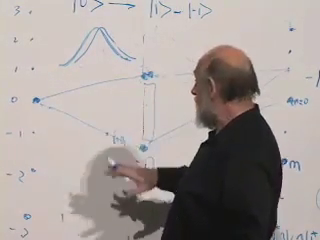
\includegraphics[width=0.68\textwidth]{lecture_06_figure_14.png}
\caption{重なり合う環境の波束と分離した環境の波束は、部分的な経路の記録と完全な経路の記録を例示する。}
\lectureframe{01:53:40}
\end{figure}

\begin{classroomqa}
\lecturetimestamp{01:50:48}
\audiencequestion{スリット近くの普通の原子は、誰も意図的に観測しなくても、通過する電子とエンタングルするのか？}
\lecturerresponse{はい。知識が作用する動詞なのではなく、物理的な相関が作用するのである。原子や周囲の気体が、その後の状態が経路を区別するのに十分なほど乱されれば、それは経路情報を記録し、干渉を抑制する。これが、そのような実験に隔離、低温、そしてしばしば光子のような弱く相互作用する粒子が必要とされる理由である。}
\end{classroomqa}

冷却は環境の自由度を基底状態近くに置き、偶発的な記録を減らす。エネルギーギャップも助けになる。入射粒子が最小の励起エネルギーを供給できなければ、環境は経路情報を保持できないかもしれない。逆に、荷電粒子はその電場を通じて近くの物質を乱しうるため、電子の干渉は特に厳しい条件を要求する。

\begin{classroomqa}
\lecturetimestamp{01:54:49}
\audiencequestion{単一電子で干渉縞を本当に得られるのか？}
\lecturerresponse{各電子は1つの局所的なヒットしか作らない。粒子を1つずつ、相互作用できないほど十分に離して送り込み、多数回の繰り返しを集める。蓄積された頻度分布が干渉縞を示す。1つの事象だけでは単なる点にすぎない。}
\end{classroomqa}

\begin{classroomqa}
\lecturetimestamp{01:55:59}
\audiencequestion{測定はエンタングルメントを破壊するのか、それとも生成するのか？}
\lecturerresponse{経路の相互作用は系と装置の間にエンタングルメントを生成し、そのエンタングルメントが選択肢間の干渉を破壊する。その後の測定は装置をさらに別の系と相関させ、残りの状態を条件づけうる。したがって、どの2つの部分系とどの干渉について論じているのかを常に明示しなければならない。}
\end{classroomqa}

\begin{classroomqa}
\lecturetimestamp{01:57:44}
\audiencequestion{相互作用を弱めて、装置が部分的な経路情報しか得ないようにできるか？}
\lecturerresponse{はい。弱い相互作用はある振幅でのみ検出器を反転させ、非直交の記録状態を残しうる。その場合、経路は部分的にしか区別できず、干渉も部分的にしか低減されない。より強い測定は、より大きな区別可能性、記録とのより強いエンタングルメント、そしてより低い縞の可視度を意味する。}
\end{classroomqa}

したがって、ここで問題となる収縮は具体的である。すなわち、経路情報が別の系に記録されたときにクロス項が失われることである。記録がなければ、振幅が加算される。完全に区別可能な記録があれば、それらの内積は消え、確率が加算される。これらの両極端の間では、測定の強さと干渉の可視度は連続的に変化する。
